\documentclass[12pt,a4paper]{article}
\usepackage{fancyhdr}
\usepackage{fontspec}
\usepackage{amsmath}
\usepackage{amssymb}
\usepackage{bm}
\usepackage{tikz}
\setmainfont{Microsoft YaHei}
\pagestyle{fancy}

\begin{document}

\fancyfoot[C]{by chinasjtu@msn.com }

\newcommand{\nl}{\newline}

\newcommand{\ntinf}{\lim\limits_{n \to \infty}}
\newcommand{\xtinf}{\lim\limits_{x \to \infty}}

\newcommand{\Atinf}{\lim\limits_{A \to \infty}}
\newcommand{\Rtinf}{\lim\limits_{R \to \infty}}

\newcommand{\ntx}[1]{\lim\limits_{n \to #1}}
\newcommand{\xtx}[1]{\lim\limits_{x \to #1}}
\newcommand{\ttx}[1]{\lim\limits_{t \to #1}} 
\newcommand{\ktx}[1]{\lim\limits_{k \to #1}} 
\newcommand{\dxtx}[1]{\lim\limits_{\Delta x \to #1}}

\newcommand{\jfab}{\int_{a}^{b}}
\newcommand{\jf}[2]{\int_{#1}^{#2}}

\newcommand{\nsum}[2]{\sum\limits_{n=#1}^{#2}}
\newcommand{\isum}[2]{\sum\limits_{i=#1}^{#2}}
\newcommand{\ksum}[2]{\sum\limits_{k=#1}^{#2}}

\newcommand{\nsuminf} {\nsum{1}{\infty}}
\newcommand{\ksuminf} {\ksum{1}{\infty}}
\newcommand{\isuminf} {\isum{1}{\infty}}





第13章 多元函数的极限连续

$13.1.欧氏空间$

$n维空间是指n维有序数组X的全体$

$X = \{(x_1,..x_n)|x_i \in R,i=1~n\}记为R^n$

$距离r(x,y)=\sqrt{\isum{1}{n}(x_i-y_i)^2}$

$(1)正定性,r(x,y) \ge 0$

$(2)对称性,r(x,y)=r(y,x)$

$(3)三角性,r(x,y) \le r(x,z)+r(y,z)$

$记R^n中\{x_k\}为x_k=(x_k^{(1)},x_k^{(2)},x_k^{(3)},...x_k^{(n)}),x_0=(x_0^{(1)},...x_0^{(n)})$

$若\ktinf r(x_k,x_0)=0,则点\{x_k\}收敛于x_0,\ktinf x_k=x_0$

$性质:极限唯一。充要条件:\ktinf x_k^{(i)}=x_0^{(0)},i=1~n$

$x_0 \in R^n,称\cup(x_0,\delta)=\{x|x \in R^n,r(x,x_0)< \delta \}为x_0$

$的\delta 邻域,\cup _0(x_0,\delta)=\cup (x,\delta) \backslash \{x_0\}$

$S的聚点全体S'(称为S的导集)\overline S = S \cup S' 称为闭包$

$闭集的等价命题:(1)对\forall \{x_n\} \subset S 若\ntinf x_n=x_0,则x_0 \in S$

$(2)S=\overline S(3) 若x \notin S,则\exists \delta >0, \cup (x,\delta) \cap S = \emptyset$

$\iff (2) 已知\overline S \supset S,S为闭集,若x \in \overline S,则x \in S或S',可见x \in S$

$由\overline S =S,设\{x_n\} \subset S,\ntinf x_n=x,若\{x_n\}中有无穷个点相异$

$则称x为聚点,x \in \overline S=S,若\{x_n\}中有限个点,\exists N \in N$

$\forall n>N,有x_n =x,于是x \in S$

$\nl$

$定理:无穷个开集之并为开集,有限个开集之交为开集$

$定理:无穷个闭集之交为闭集,有限个闭集之并为闭集$

$Cauchy定理:平面点列\{x_n\}收敛的充要条件是\{x_n\}为基本列,即\forall \epsilon>0$

$\exists N \in N:对\forall n>N,\forall p \in N 有r(x_{n+p},x_n)<\epsilon$

$\nl$

$13.2.多元函数的极限$

$二元函数D \subset R^2,\exists f:D \to R,(x,y) |\to z:f(x,y)$

$(1)设f(x,y)=\begin{cases} xsin\frac{1}{y}+ysin\frac{1}{x},xy \ne 0 \\ 0,xy=0 \end{cases}$

$|f(x,y)-0| \le |x|+|y|$

$对\forall \epsilon > 0,令\delta = \epsilon,当|x|< \delta,|y|< \delta,且x^2+y^2 \ne 0 时$

$(2) \lim\limits_{x\to \infty \atop y\to \infty} \frac{x+y}{x^2+y^2-xy}=0,0 \le |\frac{x+y}{x^2+y^2-xy}| \le |\frac{x+y}{xy}| \le \frac{1}{|x|}+\frac{1}{|y|}$

$\frac{x^2y^2}{x^2+y^2} \le  \frac{(x^2+y^2)^2}{x^2+y^2},\frac{x^2y^2}{x^2+y^2} \le \frac{x^2y^2}{2xy}  x \ne 0,y \ne 0,违反要求,只能一个不等0$

$(3)\lim\limits_{x\to 0 \atop y\to 0}\sqrt{x^2+y^2} ln(x^2+y^2)=0$

$令x=rcos \theta,yrsin \theta,则rlnr^2=2rlnr$

$当\rtx{0+} lnr·r=0,故有....$

$\nl$

$方法(1)\epsilon - \delta(2)极坐标(3)一元函数结论$

$(4)e^t < t^2, \frac{x^2+y^2}{e^{x+y}} \le \frac{e^x+e^y}{e^{x+y}}$

$\nl$

$\ntinf f(P_n)=A,P_n为D的零点,条件可减弱为 \ntinf f(P_n)存在$

$推论:在定理条件下,设E_1,E_2 \subset D 均以P_0为零点,若$

$\lim\limits_{P \to P_0 \atop P \in E_1}f(P)=A_1,\lim\limits_{P \to P_0 \atop P \in E_2}f(P)=A_2,A_1 \ne A_2,则\ptx{p_0}f(p)不存在$

$二次极限P140$

$若f(x,y)在(x_0,y_0)处有二重极限\lim\limits_{x \to x_0 \atop y \to y_0}f(x,y)=A又当x \ne x_0$

$y \to y_0时, \ytx{y_0}f(x,y)=\varphi(x),则f(x,y)在(x_0,y_0)处先y后x的二次极限存在且等于A$

$向量场$

$13.3.多元函数的连续性,$

$f(P)定义在D \subset R^2,P_0 \in D,若\forall \epsilon>0, \exists \delta >0,|f(P)-f(P_0)|< \epsilon, \forall P \in \cup(P_0,\delta) \cap D$

$称f(P)在P_0连续$

$例:f(x,y)=\begin{cases} y,x为有理数 \\ 0,x为无理数 \end{cases}在D=\{(x,0)\}上连续,在R^2 /D不连续$

$\lim\limits_{x \to x_0 \atop y \to y_0}f(x,y)=\begin{cases} y,x_0 \in Q \\ 0,x \notin Q \end{cases}故二重极限不存在$

$(x_0,0),|f(x,y)-f(x_0,0|\le|y|$

$设f(x,y)定义在D \subset R^2 上且对x连续,而对y在D上满足Lipshity条件$

$\forall (x,y')(x,y'') \in D 有|f(x,y')-f(x,y'')| \le L|y'-y''|$

$|f(x,y)-f(x_0,y_0)| \le |f(x,y)-f(x,y_0)| + |f(x,y_0)-f(x_0,y_0)|$

$\nl$

$定理1:设u=\varphi (x,y),v=\psi (x,y)在XY平面上P_0(x_0,y_0)某领域有定义$

$且在P_0处连续,又f(u,v)在uv平面上Q_0(u_0,v_0)处某领域有定义且连续$

$u_0=\varphi (x_0,y_0),v_0=\psi(x_0,y_0)则F(x,y) \triangleq f(\varphi(x,y),\psi(x,y))在点P_0处连续$

$\nl$

$\lim\limits_{x \to x_0 \atop y \to y_0}f(x,y)=A \nleftrightarrow \forall \epsilon>0,\exists \delta>0,0<|x-x_0|<\delta,0<|y-y_0|<\delta,|f(x,y)-A|< \epsilon$

$\lim\limits_{x \to x_0 \atop y \to y_0}f(x,y)=A \leftrightarrow \forall \epsilon>0,\exists \delta>0,0<max\{|x-x_0|,|y-y_0|\}<\delta,|f(x,y)-A|< \epsilon$

$\lim\limits_{x \to x_0 \atop y \to y_0}f(x,y)=A \leftrightarrow \forall \epsilon>0,\exists \delta>0,0<|x-x_0|+|y-y_0|<\delta,|f(x,y)-A|< \epsilon$

$(1)\forall \epsilon >0,\forall \theta \in [0,2\pi),\exists \delta>0,当0<r<\delta 时,有$

$|f(x_0+rcos\theta,y_0+rsin\theta)-A|<\epsilon|$

$(2)\forall \epsilon>0,\exists \delta>0,当0<r<\delta 时有$

$|f(x_0+rcos \theta ,y+rsin\theta)-A|< \epsilon,\forall \theta \in [0,2\pi]$

$\nl$

$由下列条件能否推出一致连续$

$(1)D有界,f(x,y) \in C(D),且对\forall (x,y)\in \overline D,\lim\limits_{x \to x_0 \atop y \to y_0}f(x,y)存在 ×$

$(2)D=R^2,f(x,y) \in C(R^2),且\lim\limits_{x \to x_0 \atop y \to y_0}f(x,y)存在  √$

$(3)对(x',y')(x'',y'')\in D 有|f(x',y')-f(x'',y'')|\le L_1 |x'-x''|+L_2|y'-y''| √$

$\nl$

$设f(x,y)=\frac{xy}{x+y},\lim\limits_{x \to 0 \atop y \to 0}f(x,y)不存在,令x(x^2-1)=y \to (0,0)$

$例:设f(x,y)=\frac{x^2-y^2}{x^2+y^2},(1)若f定义域为D_1=R^2\backslash \{0\},则$

$\lim\limits_{x \to 0 \atop y \to 0}f(x,y)不存在:可令y=kx$

$(2)若f定义域为D_2=\{(x,y)| |y|<x^2\}则\lim\limits_{x \to 0 \atop y \to 0}f(x,y)存在$

$依题有x \ne 0,|\frac{x^2-y^2}{x^2+y^2}-1|=\frac{2y^2}{x^2+y^2} \le \frac{2y^2}{x^2} <2x^2$

$\nl$

$例:证明\lim\limits_{x \to x_0 \atop y \to y_0}f(x,y)=A的充要条件是:对经过(x_0,y_0)的任一连续曲线$

$x=x(t),y=y(t),其中x_0=x(t_0),y=y(t_0),都有\ttx{t_0}f(x(t),y(t))=A$

$对\forall \{t_n\}(t_n \ne  t_0,t_n \to t_0)则(x(t_n),y(t_n))构成趋于$

$(x_0,y_0)的点列,利用二元函数归结原理有\ntinf f(x_n,y_n)=A$

$令F(t)=f(x(t),y(t))由\ntinf F(t_n)=A用一元函数归结原理$

$有\ttx{t_0}F(t)=A即\ttx{t_0}f(x(t),y(t))=A 反之,若有\ttx{t_0}f(x(t),y(t))=A$

$对\forall \{t_n\}(t_n \ne t_0,t_n \to t_0)连接\{x(t_n),y(t_n)\}相邻各点,构成$

$趋于(x_0,y_0)的连续折线,则由一元函数归结原理有\ntinf f(x_n,y_n)=A$

$再由二元函数归结原理有 \lim\limits_{x \to x_0 \atop y \to y_0}f(x,y)=A$

$\nl$

$称d(a,D)=inf\{|x-a||a \in R^n,\forall x \in D \subset R^n\}为点a到集合D的距离$

$证明:(1)a \in \overline D \iff d(a,D)=0(2)f(x)=d(x,D)在R^n 上一致$

$连续(3)若A,B \subset R^n 均非空,不交,且非并集,则必存在R^n上的连续函数$

$g(x)满足0 \le g(x) \le 1 且 g(x) = \begin{cases} 0,x \in A \\ 1,x \in B \end{cases} $

$(2)由定义可知 f(x) \le |\alpha -x|,\forall \alpha \in D ,x \in R^n$

$对\forall x R^n,由下确界定义,\forall \epsilon >0,\exists d_x \in D:$

$|d_x - x |< f(x)+\epsilon \to f(x)>|d_x -x|-\epsilon$

$于是对\forall x,y \in R^n,有f(y)-f(x)<|\alpha_x-y|-|\alpha_x-x|+\epsilon \le |y-x|+\epsilon$

$对换xy,f(x)-f(y) \le |x-y|+\epsilon,由\epsilon 的任意性得出|f(y)-f(x)|\le$

$(y-x)满足lipshity,故为一致连续$

$(3)构造g(x)=\frac{d(x,A)}{d(x,A)+d(x,B)} 且d(x,A)+d(x,B) \ne 0 (A,B 不交)$

$偏导数\lim\limits_{\Delta x \to 0 \atop \Delta y \to 0}f(x,y) \frac{\Delta z-dz}{\sqrt{\Delta x^2+\Delta y^2}}=0,则可微$

$考虑f=\begin{cases}\frac{xy}{\sqrt{x^2+y^2}}, x^2+y^2 \ne 0 \\ 0,x^2+y^2=0 \end{cases}$

$\nl$

$复合函数偏导法则$

$求导用树形$

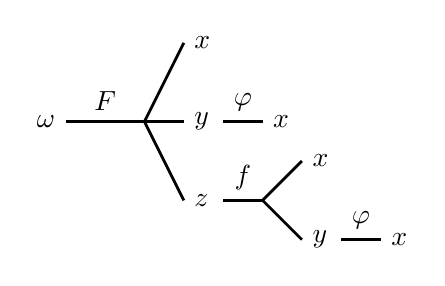
\begin{tikzpicture}[domain=1:5,line width=1pt]

\draw[-]  (0,0)--(1,0);

\draw[-]  (1,0)--(1.5,0);
\draw[-]  (1,0)--(1.5,1);
\draw[-]  (1,0)--(1.5,-1);

\draw[-]  (2,0)--(2.5,0);
\draw[-]  (2,-1)--(2.5,-1);

\draw[-]  (2.5,-1)--(3,-0.5);
\draw[-]  (2.5,-1)--(3,-1.5);

\draw[-]  (3.5,-1.5)--(4,-1.5);

\node [left] at (0,0) {$\omega$};

\node [above] at (0.5,0) {$F$};
\node [right] at (1.5,0) {$y$};

\node [right] at (1.5,1) {$x$};
\node [right] at (1.5,-1) {$z$};

\node [right] at (2.5,0) {$x$};
\node [above] at (2.25,0) {$\varphi$};

\node [above] at (2.25,-1) {$f$};

\node [right] at (3,-0.5) {$x$};
\node [right] at (3,-1.5) {$y$};

\node [above] at (3.75,-1.5) {$\varphi$};
\node [right] at (4,-1.5) {$x$};
\end{tikzpicture}

$例w=F(x,y,z),z=f(x,y),y=\varphi(x)$

$\frac{dw}{dx}=\frac{\partial F}{\partial x}+\frac{\partial F}{\partial y}\frac{dy}{dx}+\frac{\partial F}{\partial z}\frac{\partial z}{\partial x}$

$=..+...\varphi `(x)+\frac{\partial F}{\partial z}(\frac{\partial f}{\partial x}+\frac{\partial f}{\partial y}\frac{dy}{dx})$

$=\frac{\partial F}{\partial x}+\frac{\partial F}{\partial y}\varphi `(x)+\frac{\partial F}{\partial z}\frac{\partial f}{\partial x}+\frac{\partial F}{\partial z}\frac{\partial f}{\partial y}\varphi `(x)$

$\nl$

$例:利用变量替换,\zeta = x-at,\eta=x+at$

$变换方程\frac{\partial 2u}{\partial t^2}=a^2 \frac{\partial ^2u}{\partial x^2}(a \ne 0)$

$解:\frac{\partial u}{\partial x}=\frac{\partial u}{\partial \zeta}+\frac{\partial u}{\partial \eta},\frac{\partial ^2u}{\partial x^2}=\frac{\partial ^2u}{\partial \zeta^2}+2\frac{\partial ^2u}{\partial \zeta \partial \eta}+\frac{\partial ^2u}{\partial \eta^2}$

$同样的,\frac{\partial ^2u}{\partial t^2}=a^2 \frac{\partial ^2u}{\partial \zeta^2}-2a^2 \frac{\partial ^2u}{\partial \zeta \partial \eta}+a^2 \frac{\partial ^2u}{\partial \eta ^2}$

$代入原方程有 \frac{\partial ^2u}{\partial \zeta \partial \eta}=0$

$取\eta 积分, \frac{\partial \eta}{\partial \zeta}=\varphi_1(\zeta)$

$对\zeta 积分,u=\jf{}{} \varphi_1(\zeta)d\zeta+ \psi(\eta) \triangleq \psi `(\zeta)+\psi(\eta)$

$\eta = \psi `(x-at)+\psi(x+at)$

$当x,y为中间变量时,x=\varphi(\zeta,\eta,\delta),x=\psi(\zeta,\eta,\delta)$

$d^2z=d(dz)=d(\frac{\partial z}{\partial x}dx+\frac{\partial z}{\partial y}dy)$

$=d(\frac{\partial z}{\partial x})dx+\frac{\partial z}{\partial x}d^2x+d(\frac{\partial z}{\partial y})dy+\frac{\partial z}{\partial y}d^2y$

$=\frac{\partial ^2z}{\partial x^2}dx^2+2 \frac{\partial ^2z}{\partial xy}dxdy+\frac{\partial ^2z}{\partial y^2}dy^2+\frac{\partial z}{\partial x}d^2x+\frac{\partial z}{\partial y}d^2y$

$方向导数与梯度(不可微函数有方向导数)P179$

\begin{tikzpicture}[domain=1:5,line width=1pt]

\draw[->]  (0.5,0)  --  (11.5,0);
\node [above] at (6,0) {$g_2$};
\draw[->]  (11.5,-0.5)  --  (0.5,-0.5);
\node [below] at (6,-0.5) {肯定};

\draw[<-]  (0.5,0.5)  --  (5.5,10.5);
\node [right] at (3,5.5) {$f_1$};
\draw[<-]  (5,10.5)  --  (0,0.5);
\node [left] at (2.5,5.5) {$g_1,h_1$};

\draw[->]  (1,0.5)  --  (6,4);
\node [left] at (3,2.5) {$g_1$};
\draw[->]  (6,3.5)  --  (1,0);
\node [right] at (3.5,2) {肯定};

\draw[->]  (5.5,10)  --  (5.5,4);
\node [left] at (5.5,7) {肯定};
\draw[->]  (6.5,4)  --  (6.5,10);
\node [right] at (6.5,7) {$f_2$};

\draw[<-]  (7,10)  --  (12,0);
\node [left] at (9.5,5) {肯定};
\draw[->]  (8,10)  --  (13,0);
\node [right] at (10.5,5) {$f_1$};

\draw[->]  (7,4)  --  (12,0);
\node [right] at (9.5,2) {$g_2$};
\draw[<-]  (6,4)  --  (11,0);
\node [left] at (8.5,2) {肯定};

\node [above] at (6,10) {连续};
\node [above] at (6,4) {可微};
\node [left] at (0,0) {可偏导};
\node [right] at (12,0) {偏导连续};

\end{tikzpicture}

$\nl$

$f_1=\sqrt{x^2+y^2}$

$f_2=\sqrt{|xy|}$

$g_1=\begin{cases}\frac{xy}{x^2+y^2},x^2+y^2 \ne 0 \\ 0,x^2+y^2=0 \end{cases}$

$g_2=\begin{cases}(x^2+y^2)sin\frac{1}{\sqrt{x^2+y^2}},x^2+y^2 \ne 0 \\ 0,x^2+y^2=0 \end{cases}$

$h_1=\begin{cases} 1,xy \ne 0 \\ 0,xy=0 \end{cases}$

$\nl$

$求偏导方法(1)直接(2)复合链式(3)一阶形式不变(可同时得\frac{\partial z}{\partial x},\frac{\partial z}{\partial y})$

$\nl$

$z^3-3xyz=a^3(a \ne 0)求\frac{\partial ^2z}{\partial x^2}|_{(0,1)}$

$解:\frac{\partial z}{\partial x}|_{(0,1)} \frac{1}{a} 代入2z(\frac{\partial z}{\partial x})^2+z^2 \frac{\partial ^2z}{\partial x^2} 2y \frac{\partial z}{\partial x}-xy \frac{\partial ^2y}{\partial x^2}=0$

$\frac{\partial ^2z}{\partial x^2}|_{(0,1)}=0$

$\nl$

$例:u,v为新变量,w=w(u,v)为新函数,变换方程$

$\frac{\partial ^2z}{\partial x^2}-2\frac{\partial ^2z}{\partial x \partial y}+\frac{\partial ^2z}{\partial y^2}=0,u=x+y,w=\frac{y}{x},w=\frac{z}{x}$

$\frac{\partial z}{\partial x}=w+x \frac{\partial w}{\partial x}$

$=w+x(\frac{\partial w}{\partial u}\frac{\partial u}{\partial x}+\frac{\partial w}{\partial v}\frac{\partial v}{\partial x})$

$=w+x\frac{\partial u}{\partial u}- \frac{y}{x}\frac{\partial u}{\partial v}$

$\frac{\partial z}{\partial y}=x \frac{\partial u}{\partial u}+\frac{\partial w}{\partial v},从而有\frac{(x-y)^2}{x^2} \frac{\partial ^2w}{\partial v^2}=0$

$\nl$

$二、极值问题$

$记A=f_{x^2}(x_0,y_0),B=f_{xy}(x_0,y_0),C=f_{y^2}(x_0,y_0)$

$H=AC-B^2,P188$

$f(x,y)=(y-x^2)(y-2x^2)画图可知(0,0)非极值点(邻域内总有正,有负)$

$例:yx^y(1-x) < e^{-1},\forall y>0,0<x<1$

$分析:最大值在内部,解得\begin{cases} y-xy-x=0 \\ 1+ylnx=0 \end{cases}代入原式$


\end{document}

